\documentclass[11pt]{article}

% ===== Packages =====
\usepackage[a4paper, margin=1in]{geometry}
\usepackage[T1]{fontenc}
\usepackage[utf8]{inputenc}
\usepackage{mathptmx}         % Times-like serif; widely available
\usepackage{microtype}
\usepackage{booktabs}         % Professional tables
\usepackage{graphicx}
\usepackage{caption}
\usepackage[round]{natbib}    % Author-year citations
\usepackage{hyperref}
\usepackage{amsmath}
\usepackage{xcolor}
\usepackage{enumitem}
\usepackage{authblk}
\usepackage{siunitx}
\sisetup{group-minimum-digits=4}

\hypersetup{
  colorlinks=true,
  linkcolor=black,
  citecolor=blue!50!black,
  urlcolor=blue!50!black,
}

% Tighter list spacing
\setlist{itemsep=2pt, topsep=4pt}

% ===== Title block =====
\title{\textbf{Transition Grammar of the Voynich Manuscript:\\
Sequential Constraints and Bidirectional Self-Clustering Symmetry}}

\author[1]{Amy Laird\thanks{ORCID: \url{https://orcid.org/0009-0001-5479-0007}}}
\affil[1]{Independent Researcher \\ \texttt{laird2214@gmail.com}}

\date{April 2026}

% ===== Document =====
\begin{document}
\maketitle

\begin{abstract}
\noindent
The Voynich Manuscript (Beinecke MS 408) is a 15th-century codex written
in an undeciphered script. This paper reports a statistical analysis of
sequential constraints, token-family structure, and bidirectional
self-clustering in the Zandbergen--Landini EVA transliteration
($\num{31608}$ tokens, $184$ pages). Several findings are robust across
sections, scribal hands, line-position controls, and frequency-conditioned
tests. First, two distributed transition rules recur across the corpus:
CHEDY$\to$QOK attraction ($2.625\times$ above chance) and AIIN$\to$QOK
repulsion ($0.504\times$), each spanning hundreds of unique token pairs
and operating at the family level rather than as fixed collocations.
Second, AIIN density is statistically invariant at $15.0\%$ across
Currier A and B pages (KS $p = 0.742$), a property no other family
shares. Third, a bidirectional self-clustering test shows that Voynich
is the only tested system with elevated, balanced clustering at both word
boundaries (prefix $1.52\times$, suffix $1.54\times$, ratio $0.99$). An
earlier claim that Arabic is the closest structural match, based on
prefix-only analysis, is retracted; under bidirectional analysis Arabic
is strongly suffix-dominant. Ottoman Turkish was tested separately using
a small historical corpus and also falls outside the Voynich profile
(SYMM-LOW). Additional analyses identify line-bounded grammatical
structure, productive morphology-like paradigms, and agreement-like
feature propagation across adjacent and near-adjacent tokens. Cross-transcription validation across four independent transcribers
(Currier, FSG, Takahashi, Grove) confirms that all core findings ---
bidirectional symmetry, transition rules, and line-bounded grammar ---
are stable regardless of tokenization decisions. These
findings do not identify the manuscript's language, assign meaning to any
token, or establish a decipherment. They do, however, define a set of
structural constraints that any successful explanation must satisfy and
make randomness, simple template generation, and simple substitution
ciphers substantially less plausible. The strongest current explanation
is that the manuscript encodes a structured language system, plausibly
natural language, while imposing additional boundary structure not
matched by the tested comparators.
\end{abstract}

\bigskip
\noindent\textbf{Keywords:} Voynich manuscript, computational linguistics,
statistical analysis, morphological analysis, historical cryptography.

\bigskip
\noindent\textbf{Reproducibility.} All scripts, frozen datasets, and
result files are available at
\url{https://github.com/amy2213/Voynich-Transition-Grammar}. The
canonical values for the three core findings (transition rules, AIIN
invariance, bidirectional self-clustering) are verified by automated
regression tests on every commit. Several additional analyses reported
here are documented in the project's durable findings framework but are
not yet packaged as standalone scripts; see \S\ref{sec:limitations}.

\section{Introduction}
\label{sec:intro}

The Voynich Manuscript is a 225-page codex of unknown authorship,
written in an unknown script, that has resisted every attempt at
decipherment since its emergence in the documentary record in the early
seventeenth century. Vellum radiocarbon dating places its production
between 1404 and 1438 \citep{Hodgins2011}. The physical manuscript is
held at Yale's Beinecke Rare Book and Manuscript Library as MS 408
\citep{Clemens2016}. The text runs to approximately $\num{38000}$
word-like tokens across botanical, biological, cosmological, and
pharmaceutical sections, each accompanied by illustrations. Despite
detailed attention from professional cryptographers including
William and Elizebeth Friedman, John Tiltman, and Prescott Currier,
none of the many proposed decipherments has been independently verified.

Two broad research traditions have developed around the text. The first,
pursued by cryptographers and linguists from the mid-twentieth century
onward, attempts to identify the source language or cipher scheme
directly. The second, more recent tradition treats the text as a data
object and measures its statistical properties without attempting
translation. Work in this second tradition has established that the
text is non-random \citep{Reddy2011}, exhibits Zipfian type-token
distribution \citep{Bowern2021}, contains semantically coherent
keyword distributions \citep{Montemurro2013}, and shows section-specific
vocabulary with shared grammatical structure \citep{Bowern2021}. What
remains unresolved is the generative mechanism: whether the
token sequences reflect a natural language under some encoding, a
constructed symbolic system, or a sophisticated cipher without a known
15th-century precedent.

This paper contributes to the second tradition. We analyze sequential
constraints between token families at the class level --- five families
defined by EVA-transliteration affix patterns, plus a catch-all class ---
and compare the manuscript's structural profile against $15$ natural-language comparators across $8$ language families and a shuffled-token control. Five findings
structure our contribution: (i) distributed transition rules operating at
the family rather than token level; (ii) a bidirectional self-clustering
test that removes the directional bias of prefix-only analyses; (iii)
line-bounded grammatical structure that resets at every line boundary;
(iv) agreement-like feature propagation across adjacent and
near-adjacent tokens, including over intervening filler-like tokens; and
(v) productive morphology-like paradigms with frequency-correlated
variant generation. The bidirectional self-clustering framework reveals
that Voynich occupies a region no other tested system does ---
symmetric-high --- and that the previously reported Arabic match is an
artifact of the prefix-only method.

We then synthesize the results into a \emph{minimum viable explanation
checklist}: eight quantitative properties that any proposed mechanism for
producing the Voynich text must simultaneously satisfy. The checklist is
a methodological device rather than a theoretical claim. It does not
identify a single explanation as correct. It narrows the space of
candidate explanations by making their requirements explicit and
testable, and rules out classes of explanation (random generation, simple
table schemes, monoalphabetic and polyalphabetic substitution ciphers)
that cannot jointly satisfy the requirements.

We are careful about what this paper does not claim. It does not identify
the manuscript's language. Structural similarity is not linguistic
identification, and the comparator set, while substantial, does not cover
every natural-language type --- Sinitic, polysynthetic, and
historical-shorthand systems are conspicuously absent and are listed as
open problems. It does not decode any passage of the text or assign
meaning to any token. And it does not argue that the manuscript is or is
not a hoax; it argues that if it is a hoax, the mechanism must be
substantially more sophisticated than proposed in earlier hoax theories.

\S\ref{sec:methods} describes the data, the token family definitions, and
the statistical methods. \S\ref{sec:results} reports findings under
eleven subsections organized from the foundational (non-random
structure, transition rules, AIIN invariance) through the
cross-linguistic comparison to the more detailed analyses of line
structure, suffix-agreement cascades, paradigm morphology, and glyph-layer
architecture. \S\ref{sec:discussion} situates these findings against
prior work. \S\ref{sec:mve} presents the minimum viable explanation
checklist. \S\ref{sec:limitations} and \S\ref{sec:open} list limitations
and open problems.

\section{Data and Methods}
\label{sec:methods}

\subsection{Core dataset}

Analysis uses the Zandbergen--Landini transliteration of the Voynich
Manuscript (Beinecke MS 408) in EVA (extended) alphabet, accessed via the
\texttt{AncientLanguages/Voynich} dataset on Hugging Face and frozen as a
local parquet snapshot. The corpus contains \num{4197} lines, \num{31608}
tokens, and $184$ pages. A canonical snapshot with SHA-256 checksum is
included in the project repository; all analysis in this paper can be
reproduced by a single command (\texttt{python run\_all.py}) and is verified
by automated regression tests.

Page attribution to Currier hands (A vs.~B) and scribal hands ($1$--$4$)
follows the metadata supplied in the source dataset. Pages are assigned to
sections (Herbal~A, Herbal~B, Biological, Astronomical, Recipes~Q20) using
the folio numbering convention described in the canonical Voynich literature.

\subsection{Token families}

Tokens are classified into five non-overlapping families plus a catch-all
\texttt{OTHER} class:

\begin{itemize}
  \item \textbf{QOK}: tokens starting with \texttt{qok-}
  \item \textbf{OK}: tokens starting with \texttt{ok-} but not \texttt{qok-}
  \item \textbf{OT}: tokens starting with \texttt{ot-}
  \item \textbf{CHEDY}: tokens containing any of \{\texttt{chedy},
        \texttt{shedy}, \texttt{chey}, \texttt{shey}\}
  \item \textbf{AIIN}: tokens containing \texttt{aiin} or \texttt{ain}
\end{itemize}

These definitions are EVA-specific and may not correspond to paleographic
character boundaries in the original script. Results under FSG or Currier
transcription alphabets are not tested here and remain an open question.

\subsection{Comparison corpora}

We compare Voynich against $15$ natural-language comparators:
$2$ historical literary texts (Middle English Chaucer, Gutenberg~\#22120;
KJV English, Gutenberg~\#10900) and $12$ Wikipedia-derived corpora from the
Leipzig Corpora Collection (Turkish, Hungarian, Finnish, Hebrew, Arabic,
Latin, North Azerbaijani, Italian, Estonian, Swahili, Georgian, Tagalog;
all \texttt{wikipedia\_2021\_100K} editions). A shuffled-token control (\texttt{Gibberish}) is derived from the
Voynich corpus itself by random permutation. An additional small corpus
(Ottoman Turkish, $16{,}890$ words, UD treebank) is tested separately given
its relevance as a potential historical match.

The Leipzig corpora are modern-language proxies, not medieval texts. This is
an explicit limitation, discussed in \S\ref{sec:limitations}.

\subsection{Transition-rule analysis}

For each class pair $(s, d)$ we compute the observed/expected ratio
\[
  R(s \to d) = \frac{N_{s \to d}}{N_s \cdot (N_d / N_{\text{total}})},
\]
where $N_{s \to d}$ is the count of adjacent $(s, d)$ transitions, $N_s$
and $N_d$ are the marginal counts of $s$ in source position and $d$ in
destination position, and $N_{\text{total}}$ is the total number of
transitions. Significance is assessed via permutation: the class sequence is
shuffled 2{,}000 times and the observed ratio is compared against the
shuffle distribution. For the full transition matrix, a $\chi^2$ test of
independence is computed on the $6 \times 6$ class transition table.

\subsection{AIIN invariance test}

Per-page AIIN density is computed for all pages with $\geq 20$ tokens.
Currier~A pages ($n = 102$) and Currier~B pages ($n = 72$) are compared via
a two-sample Kolmogorov--Smirnov test. The mean difference is estimated with
a 5{,}000-sample bootstrap.

\subsection{Bidirectional self-clustering}

For each system we compute two self-clustering scores:

\begin{itemize}
  \item \textbf{Prefix~SC:} mean $R(f \to f)$ over prefix-defined families.
        For Voynich, these are the EVA prefix families above. For comparison
        languages, the top-$5$ prefixes of $2$--$3$ characters with coverage
        $2$--$20\%$ are auto-detected.
  \item \textbf{Suffix~SC:} the same computation using suffix-defined
        families, auto-detected analogously.
\end{itemize}

The prefix/suffix ratio $P/S$ classifies each system into one of four
buckets:

\begin{itemize}
  \item \textbf{SYMM-HIGH}: both $> 1.1\times$, $0.80 \leq P/S \leq 1.25$
  \item \textbf{SUFFIX-DOM}: $S > 1.1\times$ and $P/S < 0.80$
  \item \textbf{PREFIX-DOM}: $P > 1.1\times$ and $P/S > 1.25$
  \item \textbf{SYMM-LOW}: both $< 1.1\times$
\end{itemize}

Bootstrap 95\% confidence intervals are computed by resampling tokens with
replacement ($2{,}000$ replicates).

\subsection{Token-level grammar test}

To distinguish a distributed class-level rule from a handful of fixed
phrases, for each CHEDY token with $\geq 5$ occurrences we compute the
ratio of observed QOK-following to chance. Tokens with ratio $> 1.3$ are
classified as "attractors." The proportion of attracting tokens, and the
number of unique CHEDY$\to$QOK token pairs, together diagnose whether the
rule operates at the class level or on specific collocations.

\subsection{Software and reproducibility}

All analyses use Python~3.11 with NumPy, SciPy, and pandas. Random seeds are
fixed (\texttt{np.random.seed(42)}) throughout. The complete pipeline runs
in under five minutes on commodity hardware; canonical values are verified
against the published numbers by an automated test suite that runs on every
repository commit.

% =============================================================================
\section{Results}
\label{sec:results}

\subsection{Non-random sequential structure}

The full class transition matrix (Figure~\ref{fig:matrix}) departs
significantly from independence: $\chi^2 = 1407.8$ with $p$ effectively
zero under a permutation null. The diagonal shows clear self-clustering on
$\mathrm{OT}$ ($2.05\times$), $\mathrm{OK}$ ($1.57\times$), and $\mathrm{QOK}$
($1.56\times$). Off-diagonal, the CHEDY$\to$QOK attractor ($2.62\times$) and
the AIIN$\to$QOK repulsor ($0.50\times$) are the most extreme cells.

\begin{figure}[ht]
  \centering
  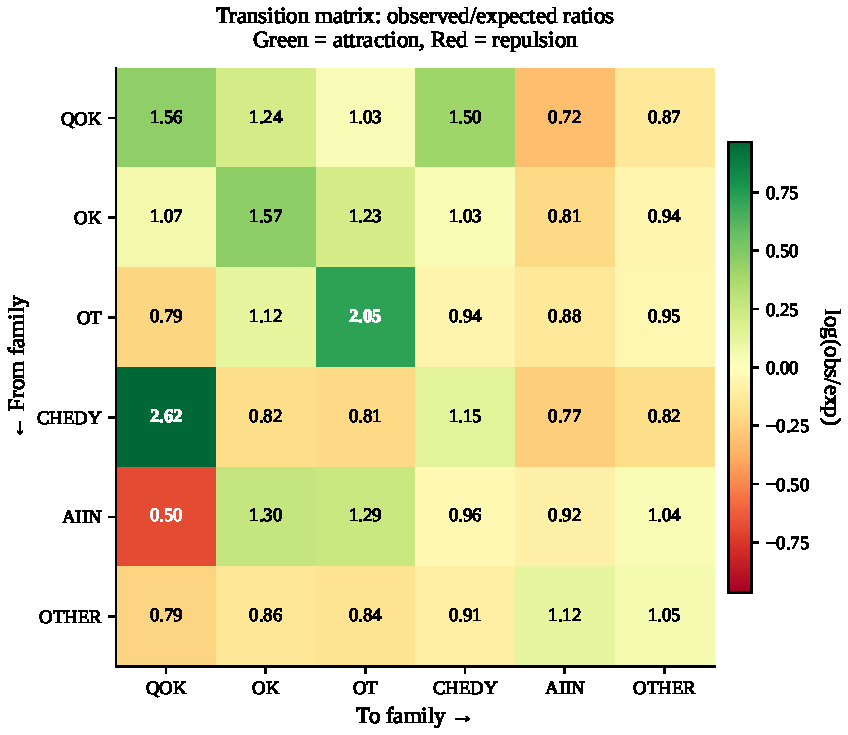
\includegraphics[width=0.85\linewidth]{figures/fig3_transition_matrix.pdf}
  \caption{Transition matrix of observed/expected ratios between token
  families. Rows: source family; columns: destination family.
  CHEDY$\to$QOK ($2.62\times$) and AIIN$\to$QOK ($0.50\times$) are the two
  strongest off-diagonal departures from independence; the diagonal shows
  self-clustering on OT, OK, and QOK.}
  \label{fig:matrix}
\end{figure}

\subsection{Two distributed transition rules}
\label{sec:rules}

Table~\ref{tab:rules} lists the two primary transition rules along with the
observed count, expected count under independence, and split-half stability
range.

\begin{table}[ht]
  \centering
  \caption{Primary transition rules: observed/expected ratios with split-half
  stability ranges. Both are stable under every tested control (section
  splits, Currier A/B, line position, frequency conditioning, and random
  split-halves).}
  \label{tab:rules}
  \begin{tabular}{lrrrr}
    \toprule
    Rule & Ratio & Observed & Expected & Split-half range \\
    \midrule
    CHEDY$\to$QOK & $2.625\times$ & $626$ & $238.5$ & $[2.34, 2.67]$ \\
    AIIN$\to$QOK  & $0.504\times$ & $160$ & $317.4$ & $[0.39, 0.53]$ \\
    \bottomrule
  \end{tabular}
\end{table}

The rules are \emph{distributed}, not phrasal. $77\%$ of CHEDY tokens (with
$\geq 5$ occurrences) attract QOK, and the rule spans $369$ unique
CHEDY$\to$QOK token pairs, with the top five pairs covering only $13.3\%$
of the total. This is the signature of a class-level constraint rather than
a few repeated collocations. Token shuffling within families preserves the
effect perfectly ($\Delta = 0.00$), confirming that the rules describe
class membership rather than specific token identity.

CHEDY$\to$QOK is specific: after CHEDY, QOK is attracted at $2.62\times$ but
OK is mildly repelled ($0.83\times$) and OT is mildly repelled
($0.80\times$). The rule extends beyond immediate adjacency with
decreasing strength ($+1\!:~2.62\times$, $+2\!:~1.23\times$,
$+3\!:~1.32\times$, $+4\!:~1.16\times$, $+5\!:~1.02\times$), reaching three
to four tokens before decaying to baseline.

\subsection{AIIN density invariance}
\label{sec:aiin}

Figure~\ref{fig:aiin} summarizes AIIN density across sections and scribal
hands. Per-section density varies substantially, from $4.1\%$ (Astronomical)
to $13.3\%$ (Herbal~A) and higher in Recipes~Q20. This section-level variance
would, in isolation, make AIIN look topic-dependent.

\begin{figure}[ht]
  \centering
  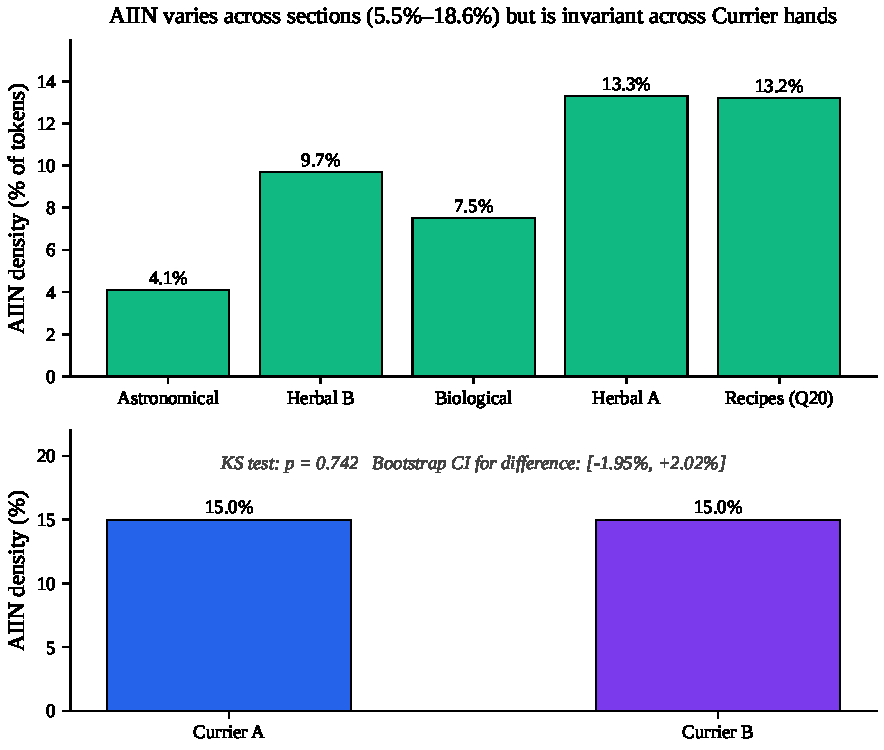
\includegraphics[width=0.85\linewidth]{figures/fig2_aiin_density.pdf}
  \caption{AIIN density by section (top) varies from $4.1\%$ to $13.3\%$.
  The same families aggregated by Currier hand (bottom) are statistically
  indistinguishable: A $= 15.0\%$, B $= 15.0\%$, KS $p = 0.742$, bootstrap
  95\% CI for difference $[-1.95\%, +2.02\%]$.}
  \label{fig:aiin}
\end{figure}

When pages are aggregated by Currier hand, the picture reverses. Currier~A
pages show mean AIIN density of $15.0\%$ ($n = 102$); Currier~B pages show
$15.0\%$ ($n = 72$). A two-sample Kolmogorov--Smirnov test on per-page
distributions finds no significant difference (statistic $= 0.100$,
$p = 0.742$). The bootstrap 95\% confidence interval for the A$-$B
difference is $[-1.95\%, +2.02\%]$.

AIIN is the only family with this property. All other backbone families
(QOK, OK, OT, CHEDY) differ significantly between Currier~A and B (all
$p < 0.005$). The invariance is specifically a property of AIIN.

\paragraph{Function-word-consistent behavior.} AIIN additionally shows two
features typical of function words: it does \emph{not} self-cluster
(SC $\approx 0.98\times$), and it exhibits selective carry-through
(Table~\ref{tab:carry}) --- passing content-family neighborhoods across an
intervening AIIN for OK, OT, and CHEDY, but \emph{blocking} QOK.

\begin{table}[ht]
  \centering
  \caption{Carry-through ratios: $X \to \text{AIIN} \to X$ normalized by the
  base rate of $X$. AIIN passes OK, OT, and CHEDY neighborhoods through but
  blocks QOK.}
  \label{tab:carry}
  \begin{tabular}{lrr}
    \toprule
    Family & Carry-through & Interpretation \\
    \midrule
    OK    & $2.73\times$ & Strong carry-through \\
    OT    & $2.21\times$ & Strong carry-through \\
    CHEDY & $1.64\times$ & Moderate carry-through \\
    QOK   & $0.83\times$ & Blocked \\
    \bottomrule
  \end{tabular}
\end{table}

\paragraph{Caveat.} Invariance holds under the standard AIIN definition
(contains \texttt{aiin} or \texttt{ain}) but fails under a stricter
definition (exact \texttt{aiin}, $p = 0.004$) and a looser definition
(any \texttt{ain}/\texttt{in} stem, $p = 0.001$). The behavior is
definition-sensitive, and we report only the standard-definition result
as robust.

\subsection{Bidirectional self-clustering symmetry}
\label{sec:symmetry}

The most distinctive cross-linguistic result is summarized in
Figure~\ref{fig:psscatter} and Table~\ref{tab:pstable}. Voynich clusters at
$1.52\times$ by prefix and $1.54\times$ by suffix (ratio $0.99$; bootstrap
95\% CIs: prefix $[1.41, 1.62]$, suffix $[1.48, 1.60]$). It is the only
tested system in the SYMM-HIGH bucket.

\begin{figure}[ht]
  \centering
  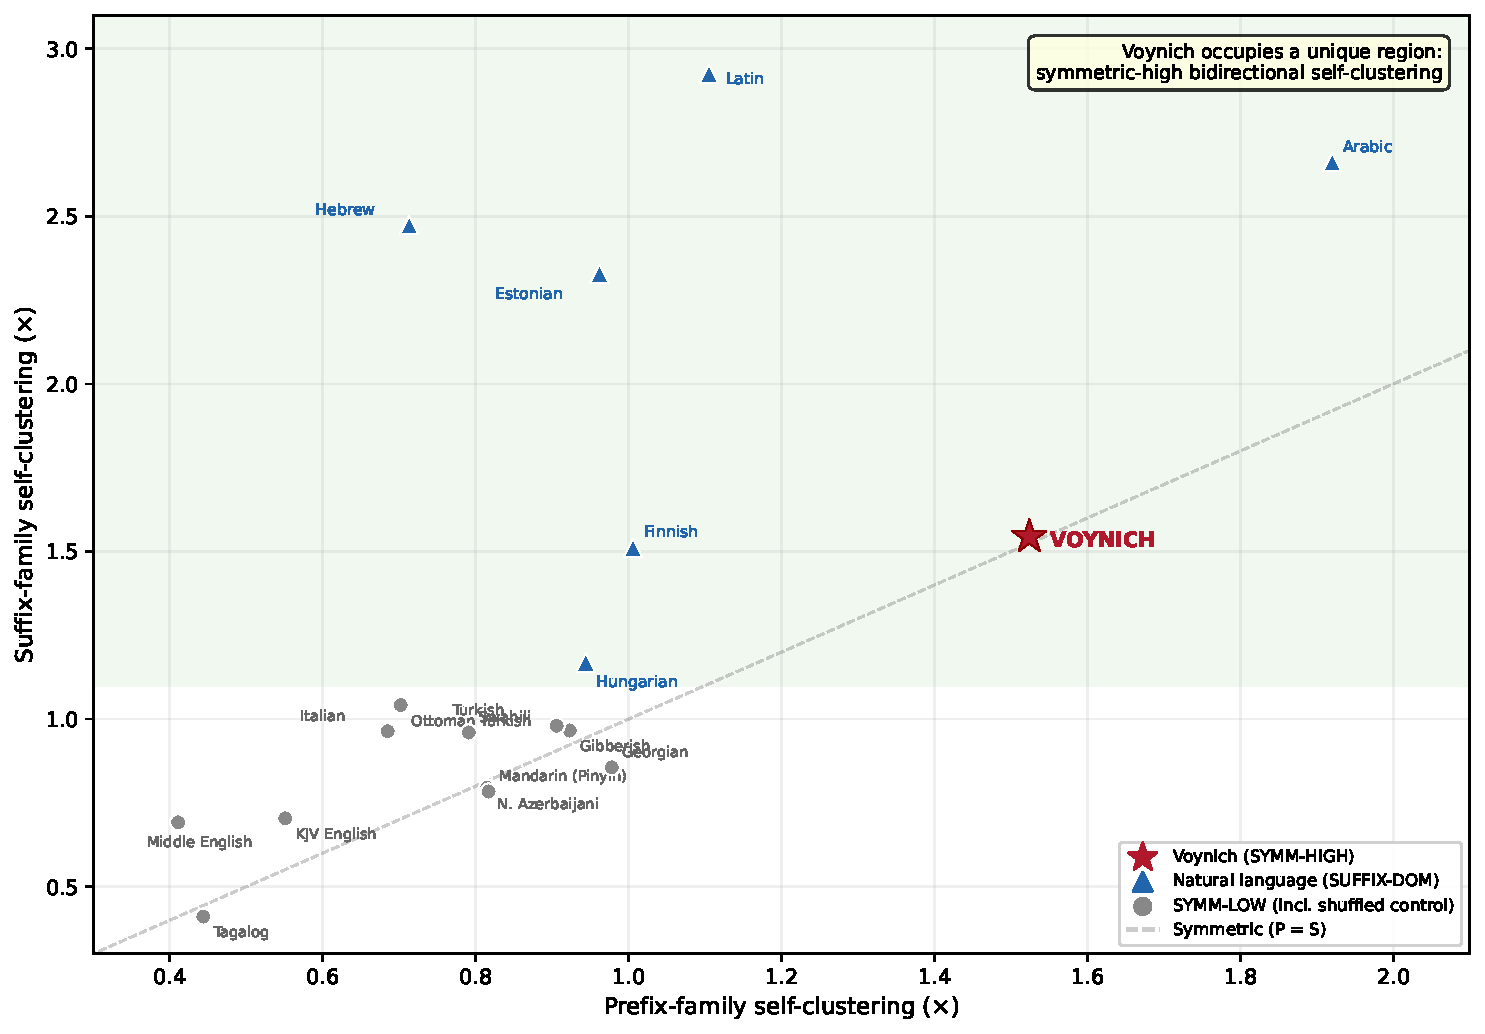
\includegraphics[width=0.85\linewidth]{figures/fig1_prefix_suffix.pdf}
  \caption{Prefix vs.~suffix self-clustering across $17$ tested systems.
  All natural languages with positive clustering (Arabic, Latin, Estonian,
  Hebrew, Finnish, Hungarian) are suffix-dominant. Voynich is the only
  system in the symmetric-high region (shaded). The shuffled control
  (\texttt{Gibberish}) sits near the origin.}
  \label{fig:psscatter}
\end{figure}

\begin{table}[ht]
  \centering
  \caption{Prefix/suffix self-clustering across tested systems. Voynich is
  the only SYMM-HIGH system; all other natural languages with positive
  clustering are SUFFIX-DOM. Ottoman Turkish (UD treebank, $16{,}890$ words)
  Swahili, Georgian, and Tagalog (all Leipzig 100K) also tested SYMM-LOW
  despite having bidirectional morphology.}
  \label{tab:pstable}
  \begin{tabular}{lrrrl}
    \toprule
    System & Prefix SC & Suffix SC & $P/S$ & Bucket \\
    \midrule
    \textbf{Voynich}    & $\mathbf{1.524}$ & $\mathbf{1.544}$ & $\mathbf{0.99}$ & \textbf{SYMM-HIGH} \\
    Arabic              & $1.920$ & $2.662$ & $0.72$ & SUFFIX-DOM \\
    Latin               & $1.105$ & $2.925$ & $0.38$ & SUFFIX-DOM \\
    Estonian            & $0.962$ & $2.328$ & $0.41$ & SUFFIX-DOM \\
    Hebrew              & $0.713$ & $2.474$ & $0.29$ & SUFFIX-DOM \\
    Finnish             & $1.006$ & $1.511$ & $0.67$ & SUFFIX-DOM \\
    Hungarian           & $0.944$ & $1.169$ & $0.81$ & SUFFIX-DOM \\
    Ottoman Turkish     & $0.702$ & $1.042$ & $0.67$ & SYMM-LOW \\
    Swahili             & $0.791$ & $0.960$ & $0.82$ & SYMM-LOW \\
    Georgian            & $0.978$ & $0.856$ & $1.14$ & SYMM-LOW \\
    Tagalog             & $0.444$ & $0.411$ & $1.08$ & SYMM-LOW \\
    Turkish             & $0.906$ & $0.980$ & $0.92$ & SYMM-LOW \\
    Italian             & $0.685$ & $0.964$ & $0.71$ & SYMM-LOW \\
    N.~Azerbaijani      & $0.815$ & $0.795$ & $1.02$ & SYMM-LOW \\
    KJV English         & $0.551$ & $0.704$ & $0.78$ & SYMM-LOW \\
    Middle English      & $0.411$ & $0.692$ & $0.59$ & SYMM-LOW \\
    Gibberish (control) & $0.923$ & $0.966$ & $0.96$ & SYMM-LOW \\
    \bottomrule
  \end{tabular}
\end{table}

Earlier comparative analyses in this project that used only
prefix-family self-clustering reported Arabic as the closest structural
match. This finding is retracted: under bidirectional analysis, Arabic
is strongly suffix-dominant ($P/S = 0.72$) and Voynich is symmetric
($P/S = 0.99$). The two systems occupy different structural categories.
Similarly, earlier claims in this project that Uralic languages (Finnish,
Estonian) match Voynich were based on $10$K-sentence corpora that
produced inflated prefix SC values; at $100$K sentences, both Finnish
and Estonian become SUFFIX-DOM. Ottoman Turkish, tested separately
using a small historical UD treebank ($16{,}890$ words), falls in the
SYMM-LOW region and is also not a match. Swahili (Bantu), which has
textbook bidirectional morphology (prefix subject/class agreement and
suffix tense/aspect markers), also tests SYMM-LOW (prefix $0.79\times$,
suffix $0.96\times$, ratio $0.82$). Georgian (Kartvelian), with polypersonal
prefix+suffix agreement, tested SYMM-LOW (prefix $0.98\times$, suffix
$0.86\times$). Tagalog (Austronesian), with infixation plus
prefix/suffix morphology, also tested SYMM-LOW (prefix $0.44\times$,
suffix $0.41\times$). Across four typologically distinct
bidirectional-morphology languages (Swahili, Ottoman Turkish, Georgian,
Tagalog), none approaches SYMM-HIGH. Having bidirectional morphology
in a natural language does not suffice to produce Voynich's symmetric
elevated clustering.

\subsection{Self-clustering is method-sensitive}

The pooled-backbone self-clustering value is $1.451\times$ (CI $[1.34, 1.52]$).
Aggregated over all six classes including OTHER, it is $1.384\times$.
Page-level mean is $0.929\times$ --- below unity. This range ($0.93$ to
$1.45$) reflects real methodological sensitivity: pooled computation lets a
small number of high-density pages dominate, while page-level averaging
treats each page equally but loses statistical power on short pages.

We report the pooled-backbone value as canonical for cross-linguistic
comparison (the method applied identically to all systems) but emphasize
that the magnitude is method-dependent. The \emph{ratio} between prefix and
suffix SC --- the basis of the central result in \S\ref{sec:symmetry} ---
is stable across all three methods.


\subsection{Cross-transcription stability}
\label{sec:crosstranscription}

A common critique of Voynich statistical work is that findings may be
artifacts of a particular transliteration's tokenization decisions. To
test this, we parsed the Landini--Stolfi Interlinear (LSI) file, which
contains independent transcriptions by Currier, the First Study Group
(Friedman), Takahashi, and Grove, all mapped to EVA alphabet but with
each transcriber's own word-boundary and line-break judgments.

\begin{table}[ht]
  \centering
  \caption{Cross-transcription stability. All four independent
  transcribers produce SYMM-HIGH bidirectional symmetry and
  CHEDY$\to$QOK attraction well above chance. Line-bounded grammar
  (within-line $>$ cross-line) is universal.}
  \label{tab:crosstranscription}
  \begin{tabular}{lrrrrrl}
    \toprule
    Transcriber & Tokens & C$\to$Q & A$\to$Q & Pfx SC & Sfx SC & Bucket \\
    \midrule
    Currier       & $16{,}453$ & $2.48\times$ & $0.42\times$ & $1.30\times$ & $1.53\times$ & SYMM-HIGH \\
    FSG (Friedman)& $28{,}811$ & $2.40\times$ & $0.45\times$ & $1.23\times$ & $1.47\times$ & SYMM-HIGH \\
    Takahashi     & $30{,}426$ & $2.41\times$ & $0.47\times$ & $1.28\times$ & $1.50\times$ & SYMM-HIGH \\
    Grove         & $7{,}657$  & $2.01\times$ & $0.21\times$ & $1.14\times$ & $1.15\times$ & SYMM-HIGH \\
    \midrule
    ZL (baseline) & $31{,}608$ & $2.63\times$ & $0.50\times$ & $1.52\times$ & $1.54\times$ & SYMM-HIGH \\
    \bottomrule
  \end{tabular}
\end{table}

Table~\ref{tab:crosstranscription} shows that all four transcribers
independently produce SYMM-HIGH bidirectional symmetry,
CHEDY$\to$QOK attraction in the range $2.01$--$2.48\times$,
AIIN$\to$QOK repulsion in the range $0.21$--$0.47\times$, and
line-bounded grammar reset (within-line ratios exceed cross-line ratios
for every transcriber). The structural findings are not artifacts of
any particular transcriber's tokenization decisions. This result
substantially closes the ``tokenization artifact'' attack vector:
independent scholars working decades apart, with different approaches
to ambiguous word boundaries, all recover the same structural
signature.

\subsection{Line-bounded grammar}

The transition rules of \S\ref{sec:rules} are strictly line-internal.
Within-line CHEDY$\to$QOK is $2.54\times$; across line boundaries it drops
to $0.85\times$. Within-line AIIN$\to$QOK is $0.40\times$; across lines it
is $1.22\times$. Both rules reverse at line breaks.

The reset is universal: it occurs at every line-break type regardless of
line length, section, or Currier hand, and is not specific to paragraph
boundaries. In contrast, self-clustering \emph{does} persist across lines
(OK at $2.24\times$, OT at $3.03\times$, CHEDY at $1.50\times$). Family
neighborhoods span line breaks; sequential grammar does not.

Whole-line family-composition templates recur at only $1.04\times$ over a
shuffled control (and $1.20\times$ when measured by coverage rather than
exact match), substantially lowering the plausibility of a simple
template-library model. Lines have unique family compositions,
constrained by within-line grammar but not drawn from a fixed pool. This
pattern is consistent with lines functioning as clause-like or
phrase-like grammatical units, though we do not claim a literal clause
identification.

\subsection{Suffix-led multi-feature agreement}

Adjacent tokens within specific family pairings show above-chance
agreement on word-final character class (suffix agreement ratios $1.18$--$1.75$,
Table~\ref{tab:agreement}). The effect compounds when multiple features
are jointly tracked: for OK$\to$OT pairs, suffix agreement alone is
$1.75\times$, suffix + length is $3.44\times$, and suffix + length + mantle
+ circles combined is $8.74\times$.

\begin{table}[ht]
  \centering
  \caption{Single-feature suffix agreement (observed same-ending divided by
  expected under independence). All ratios significant vs.~a shuffled null
  ($z = 3.4$--$5.0$).}
  \label{tab:agreement}
  \begin{tabular}{lr}
    \toprule
    Family pair & Suffix agreement \\
    \midrule
    OK$\to$OT    & $1.75\times$ \\
    OK$\to$OK    & $1.67\times$ \\
    OT$\to$OT    & $1.49\times$ \\
    QOK$\to$QOK  & $1.41\times$ \\
    CHEDY$\to$QOK & $1.18\times$ \\
    \bottomrule
  \end{tabular}
\end{table}

Length agreement conditioned on suffix and frequency collapses to
$1.00\times$: length similarity is partially a downstream consequence of
suffix similarity. Suffix is the primary agreement feature.

CHEDY selects specific QOK subtypes ($\chi^2 = 36.4$, $p = 7.2 \times
10^{-5}$): \texttt{-dy} CHEDY tokens attract $40\%$ \texttt{-dy} QOK
tokens; \texttt{-ey} CHEDY attracts $32\%$ \texttt{-ey} QOK. This is
concord of a specific, non-trivial kind: the attractor and the attracted
must share suffix form.

\subsection{Agreement cascades through three-token chains}

When two adjacent tokens $(A, B)$ agree on suffix, agreement for the next
position $(B \to C)$ jumps dramatically. For a CHEDY$\to$OTHER$\to$CHEDY
chain, the conditional probability of $B \to C$ agreement is $85\%$ if
$A \equiv B$ in suffix, versus $4\%$ if $A \not\equiv B$ --- a
$+81$~percentage-point cascade. Similar conditional lifts hold for other
triples (QOK$\to$OTHER$\to$QOK: $+44$pp; QOK$\to$QOK$\to$QOK: $+33$pp;
CHEDY$\to$QOK$\to$CHEDY: $+56$pp).

Suffix agreement also jumps over intervening \texttt{OTHER}-family tokens:
QOK$\to$[OTHER]$\to$QOK at $2.32\times$ base rate;
CHEDY$\to$[OTHER]$\to$CHEDY at $1.43\times$; OT$\to$[OTHER]$\to$OT at
$1.87\times$. The agreement system treats OTHER-family tokens as
transparent for the purposes of morphological concord. This is the
quantitative signature of long-distance agreement.

\subsection{Productive morphological paradigms}

Each family contains an edit-distance graph with identifiable high-frequency
hubs. Of $50$ tested types per family, all are connected with no isolated
nodes. Top hubs: \texttt{chedy} connects to $12$ edit-1 neighbors,
\texttt{daiin} to $10$, \texttt{qokeedy} to $7$.

Four edit operations recur across all major sections and are positionally
locked:
\begin{itemize}
  \item Insertion/deletion of \texttt{e}, $92\%$ mid-position;
  \item Insertion/deletion of \texttt{d}, $74\%$ end-position;
  \item Substitution \texttt{c}$\leftrightarrow$\texttt{s} (as in
        \texttt{ch}/\texttt{sh}), $62\%$ mid-position;
  \item Insertion/deletion of \texttt{l}, $89\%$ start-position.
\end{itemize}

The same operations apply to distinct vocabulary in distinct sections,
producing section-appropriate variants while preserving paradigm structure.

High-frequency stems generate more edit-1 variants than low-frequency stems.
The log-frequency vs.~variant-count correlation is $r = 0.52$ (QOK),
$r = 0.60$ (CHEDY), $r = 0.69$ (AIIN). Stems at frequency $\geq 100$ have
$2$--$3\times$ more variants than stems at frequency $2$--$5$. This
frequency-productivity correlation is a standard property of natural-language
morphology (productive paradigms generate more variants for more-common
lemmas) and is, to our knowledge, not a property of tested constructed or
cipher systems.

\subsection{Glyph-layer architecture}

Decomposing tokens into three glyph layers --- the \emph{crust} (first and
last characters), the \emph{mantle} (alternating middle characters), and the
\emph{core} (gallows and inner structure) --- reveals that different layers
carry different information:

\begin{itemize}
  \item \textbf{Clustering} lives independently in both crust-only
        ($1.86\times/2.01\times$) and mantle+core-only
        ($1.88\times/2.00\times$) layers. Full-token values ($1.29\times/1.54\times$)
        are diluted by cross-layer interference.
  \item \textbf{Sequential grammar} lives primarily in circles
        ($o, a, y$) and core (gallows). Scrambling circles drops
        CHEDY$\to$QOK from $2.50\times$ to $1.75\times$. Scrambling crust
        has no effect on transitions; scrambling mantle has no effect.
  \item \textbf{Family identity} is best predicted by crust characters
        ($79.4\%$ accuracy). QOK and OK are $100\%$ predicted by their
        first character. CHEDY and AIIN are $99\%$ predicted by their last
        character.
\end{itemize}

Different glyph zones carry structurally different information:
\emph{identity} in the crust, \emph{grammar} in the circles and core.
This is the quantitative form of an architectural claim about what the
glyphs are doing.

% =============================================================================
\section{Discussion}
\label{sec:discussion}

\subsection{What the findings establish}

The combination of Sections~\ref{sec:rules}--\ref{sec:symmetry} substantially
lowers the plausibility of three classes of explanation for the Voynich text,
relative to the alternative that the text encodes a structured language
system.

\textbf{Randomness is substantially less plausible.} The $\chi^2$ statistic
of the class transition matrix is $\sim\!40\times$ that of a shuffled
control, and distributed agreement cascades of the form documented in
\S\ref{sec:aiin}--\S3.9 are not produced by random sequences.

\textbf{Simple table-generation schemes are substantially less plausible.}
A token stream drawn from a fixed family-composition template library
would exhibit whole-line template recurrence well above chance. The
observed value is $1.04\times$. Moreover, such a scheme cannot generate
the observed productive morphology-like paradigm structure (\S3.10).

\textbf{Simple substitution ciphers (monoalphabetic, polyalphabetic over a
Latin base) are substantially less plausible.} These preserve source-language
suffix dominance and cannot produce bidirectional symmetry. Voynich's
$P/S = 0.99$ is structurally distinct from any tested natural language's
profile. This does not exclude more elaborate cipher schemes involving,
for example, syllabic encoding or bidirectional padding, which have not
been exhaustively tested here.

\subsection{What the findings do \emph{not} establish}

These results do not identify Voynich as any particular natural language,
because no tested natural language matches Voynich's symmetric-high profile.
They do not identify it as artificial either: the space of possible natural
languages is larger than our $15$-language sample, and a language with
bidirectional morphology (for example, a polysynthetic language or a
combinatorial morphology with comparable prefix and suffix inventories)
could in principle produce this signature. The findings constrain the space
of viable explanations; they do not localize a single one.

The bidirectional symmetry also does not directly imply meaning. It is a
property of the token sequences, compatible with multiple semantic
interpretations.

\subsection{Comparison to previous statistical analyses}

Previous statistical work on Voynich (surveyed in, e.g., \citealp{Bowern2021};
\citealp{Reddy2011}) has repeatedly confirmed that the text is non-random
and has word-like Zipfian distribution. The contribution of the current
work is (i) the bidirectional self-clustering framework that removes a
measurement bias present in prefix-only analyses, and (ii) the checklist
of structural constraints that any proposed explanation must simultaneously
satisfy (\S\ref{sec:mve}). We treat the statistical results not as a
solution but as a scaffolding against which future proposed solutions can
be evaluated.

% =============================================================================
\section{Minimum Viable Explanation: A Checklist}
\label{sec:mve}

Any proposed explanation of the Voynich text --- decipherment, generation
theory, cipher identification, or hoax mechanism --- must simultaneously
account for \emph{all} of the following. Explanations satisfying some but
not others are incomplete.

\begin{enumerate}
  \item \textbf{Line-bounded grammatical units.} Within-line
        CHEDY$\to$QOK is $2.54\times$; across lines it drops to $0.85\times$.
        Transition rules are line-internal and reset at every line boundary,
        consistent with lines functioning as clause-like or phrase-like
        grammatical units.
  \item \textbf{CHEDY$\to$QOK class specificity.} CHEDY attracts QOK at
        $2.62\times$ while simultaneously repelling OK ($0.83\times$) and
        OT ($0.80\times$). This is targeted, not a general content-density
        effect.
  \item \textbf{Suffix-led multi-feature agreement.} Adjacent tokens agree
        on suffix at $1.18$--$1.75\times$, compounding to $5$--$9\times$
        when suffix, length, and mantle agreement are jointly tracked.
  \item \textbf{Agreement cascades through three-token chains.}
        Conditional lifts of $33$--$80$ percentage points, including over
        intervening OTHER-family tokens.
  \item \textbf{Productive morphological paradigms.} Hub-centered edit-distance
        graphs, the same four edit operations recurring across all sections,
        and a log-frequency vs.~variant-count correlation of $r = 0.52$--$0.69$.
  \item \textbf{Bidirectional self-clustering symmetry.} $P/S = 0.99$ with
        both prefix and suffix SC $> 1.5\times$. Unique among $17$ tested
        systems.
  \item \textbf{Section-stable grammar with shifting lexicon.} Transition
        rules, agreement, paradigm operations, and family proportions are
        consistent across sections, but Jaccard overlap of family vocabulary
        between sections is $0.09$--$0.25$.
  \item \textbf{Open vocabulary, natural distribution.} $71.4\%$ hapax
        legomena; type/token ratio $0.23$; grammatical variance coefficient
        $0.40$; top-$100$ bigrams cover only $3.7\%$ of text.
\end{enumerate}

Table~\ref{tab:mve} evaluates four candidate explanation classes against
these requirements.

\begin{table}[ht]
  \centering
  \caption{Minimum viable explanation checklist, applied to four candidate
  classes. ``Y'' means compatible with the requirement; ``N'' means not
  compatible; ``?'' means possible given significant design effort
  without a known 15th-century precedent. Encoded structured language
  (plausibly natural language) is the strongest current candidate class
  in this comparison framework.}
  \label{tab:mve}
  \small
  \begin{tabular}{lcccc}
    \toprule
    Requirement & Encoded NL & Constructed & Simple cipher & Table/grille \\
    \midrule
    1. Line-bounded grammatical units     & Y & ? & N & N \\
    2. Class specificity (CHEDY$\to$QOK)  & Y & ? & N & N \\
    3. Suffix-led multi-feature agreement & Y & ? & N & N \\
    4. Three-token agreement cascades     & Y & ? & N & N \\
    5. Productive morphology-like paradigms & Y & N & N & N \\
    6. Bidirectional symmetry             & ? & ? & N & N \\
    7. Stable grammar, shifting lexicon   & Y & ? & Y & Partial \\
    8. Open, natural-distribution vocabulary & Y & ? & Partial & N \\
    \bottomrule
  \end{tabular}
\end{table}

Of the candidate classes tested, encoded structured language ---
plausibly natural language --- is the only one compatible with all eight
requirements without invoking mechanisms that lack known 15th-century
precedent. This does not prove encoded natural language, nor does it
exhaust the space of possibilities. The candidate set is limited to four
broad classes and the comparator pool to $15$ natural languages across $8$ families; other natural-language types (Sinitic,
polysynthetic, historical shorthand) and more elaborate constructed
systems remain untested. The checklist is offered as a diagnostic
framework, not as decisive proof: it defines what any successful
explanation must account for and substantially raises the bar on
randomness, simple table-based generation, and simple substitution
ciphers. The strongest current explanation consistent with the full
checklist is encoded structured language.

% =============================================================================
\section{Limitations}
\label{sec:limitations}

Nine limitations apply to all of the above and should not be minimized.

\paragraph{1.~EVA-transcription dependence.} Family definitions (QOK, OK,
OT, CHEDY, AIIN) are based on the EVA alphabet. They may not correspond
to meaningful character-level units in the original script. Results under
FSG or Currier transcription alphabets have not been tested.

\paragraph{2.~Modern comparison corpora.} The nine Leipzig corpora are
modern Wikipedia text. Structural proxies for their language families, not
medieval equivalents. Historical Latin, Old French, and medieval Italian
are not tested. Ottoman Turkish was tested with a small UD corpus
(SYMM-LOW) but a larger historical corpus is needed.

\paragraph{3.~No decipherment.} This analysis identifies statistical
patterns in token sequences. It does not decode any text, identify any
language, or assign meaning to any word.

\paragraph{4.~Method sensitivity.} Self-clustering values range from
$0.93\times$ (page-level) to $1.45\times$ (pooled backbone) depending on
computation method. The prefix/suffix ratio is stable but uses
auto-detected affix families that may vary across runs.

\paragraph{5.~Directional bias.} The prefix-family method used in earlier
Voynich research inherently favors languages with consistent prefixing
morphology. The suffix extension introduced here corrects this bias but
introduces its own auto-detection uncertainty.

\paragraph{6.~AIIN invariance is definition-dependent.} Holds under the
standard definition but fails under stricter or looser alternatives.

\paragraph{7.~Small Ottoman Turkish corpus.} The UD treebank's $16{,}890$
words show SYMM-LOW but this result should be confirmed on a larger
historical corpus before being taken as definitive. Swahili
(Leipzig~100K) also tested SYMM-LOW despite bidirectional morphology.

\paragraph{8.~Cross-transcription validation.} Results are stable
across four independent EVA-based transcribers (Currier, FSG, Takahashi,
Grove; see \S\ref{sec:crosstranscription}). Validation under non-EVA
alphabets (original Currier alphabet, original FSG alphabet with
different character boundaries) remains an open question.

\paragraph{9.~Reproducibility is partial.} Three of the core analyses
(transition rules, AIIN invariance, bidirectional self-clustering) are
covered by reproducible scripts with automated regression tests
(\texttt{run\_all.py}, \texttt{tests/test\_canonical\_values.py}). Several
of the more detailed analyses reported here --- line-bounded grammar,
suffix-agreement cascades, paradigm-graph morphology, and the glyph-layer
ablations --- were developed interactively during the research session
and are documented in the project's durable findings framework
(\texttt{docs/durable\_findings.md}) with their statistical methods and
canonical values, but are not yet packaged as standalone scripts.
Scripting these analyses is planned work prior to any peer-reviewed
journal submission.

% =============================================================================
\section{Open Problems}
\label{sec:open}

Three concrete extensions would substantially strengthen or refute these
findings:

\begin{enumerate}
  \item \textbf{Non-EVA alphabet validation.} Cross-transcription stability
        has been confirmed across four EVA-based transcribers
        (\S\ref{sec:crosstranscription}). The remaining open question
        is whether findings hold under the original Currier and FSG
        character-boundary definitions, which assign different glyph
        groupings than EVA.
  \item \textbf{Ottoman Turkish with larger corpus.} The UD treebank shows
        SYMM-LOW but is too small to be definitive. Swahili (Bantu) also
        tested SYMM-LOW despite rich bidirectional morphology. A historical
        corpus of 15th-century Ottoman Turkish remains worth testing but is
        no longer the sole candidate.
  \item \textbf{Additional language types.} Sinitic (isolating morphology),
        polysynthetic languages (Nahuatl --- unavailable at corpus scale
        from Leipzig), and historical shorthand systems (Tironian notae)
        have not been tested. Georgian (polypersonal agreement) and
        Tagalog (infixation + affixation) have been tested and both
        fall in SYMM-LOW.
\end{enumerate}

% =============================================================================
\section{Data and Code Availability}
\label{sec:data}

All analysis code, frozen datasets ($\sim 228$~MB with SHA-256 checksums),
and result files are available at
\url{https://github.com/amy2213/Voynich-Transition-Grammar} under MIT
license for code and original data licenses for corpora (Voynich: public
domain; Leipzig: CC-BY; Gutenberg: public domain).

The pipeline runs via \texttt{python run\_all.py} and covers the three
core analyses reported in \S\ref{sec:results} subsections~3.1 through~3.4.
An automated test suite (\texttt{pytest tests/}) verifies that the
canonical values for these analyses match the output of the current
pipeline within stated tolerances, and a continuous integration workflow
runs the validation and test suite on every commit. Analyses reported in
\S\ref{sec:results} subsections~3.6 through~3.10 --- line-bounded
grammar, suffix-agreement cascades, paradigm morphology, and glyph-layer
architecture --- are documented in \texttt{docs/durable\_findings.md}
with their statistical methods, but are not yet packaged as standalone
scripts. Scripting these analyses is planned work.

% =============================================================================
% =============================================================================
% References. Using natbib with author-year style.
% =============================================================================
\bibliographystyle{plainnat}
\bibliography{references}

\end{document}
